\section{Постановка задачи}

\begin{frame}
    \frametitle{Постановка задачи}
    \begin{figure}
        \centering
        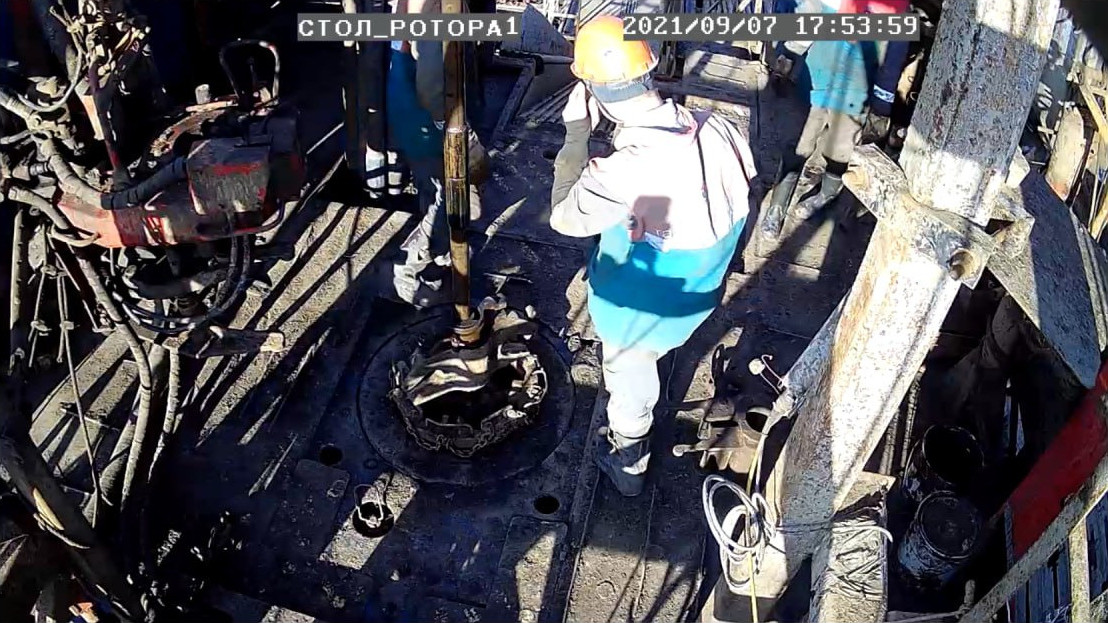
\includegraphics[width=1.0\textwidth,keepaspectratio]{problem_formulation_1}
    \end{figure}
\end{frame}

\begin{frame}
    \frametitle{Постановка задачи}
    \begin{figure}
        \centering
        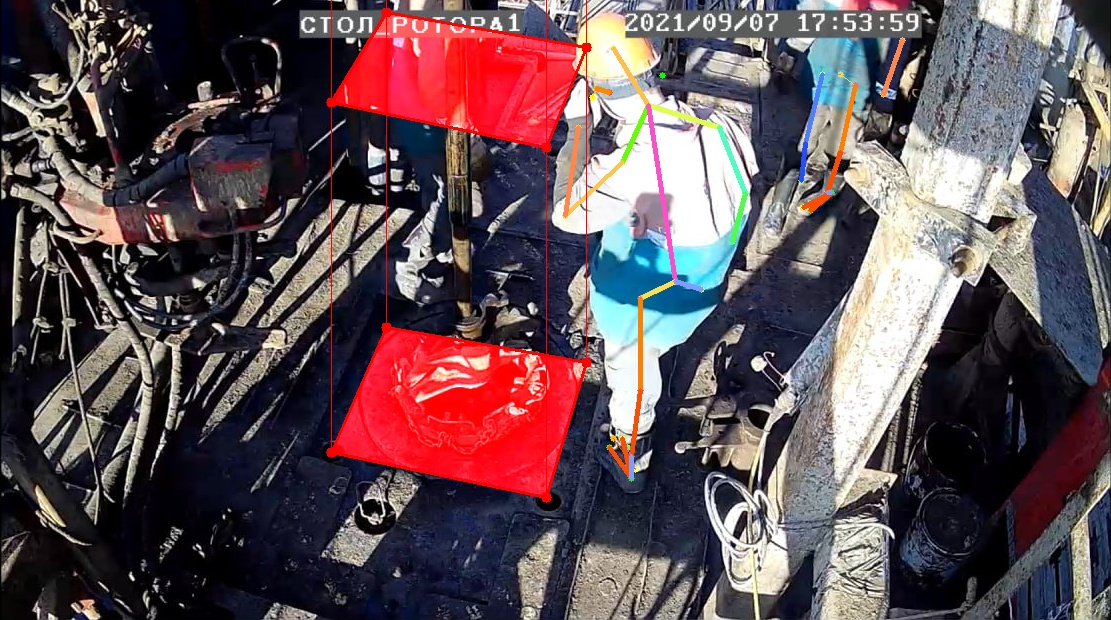
\includegraphics[width=1.0\textwidth,keepaspectratio]{problem_formulation_2}
    \end{figure}
\end{frame}

\begin{frame}
    \frametitle{Постановка задачи}
    \begin{figure}
        \centering
        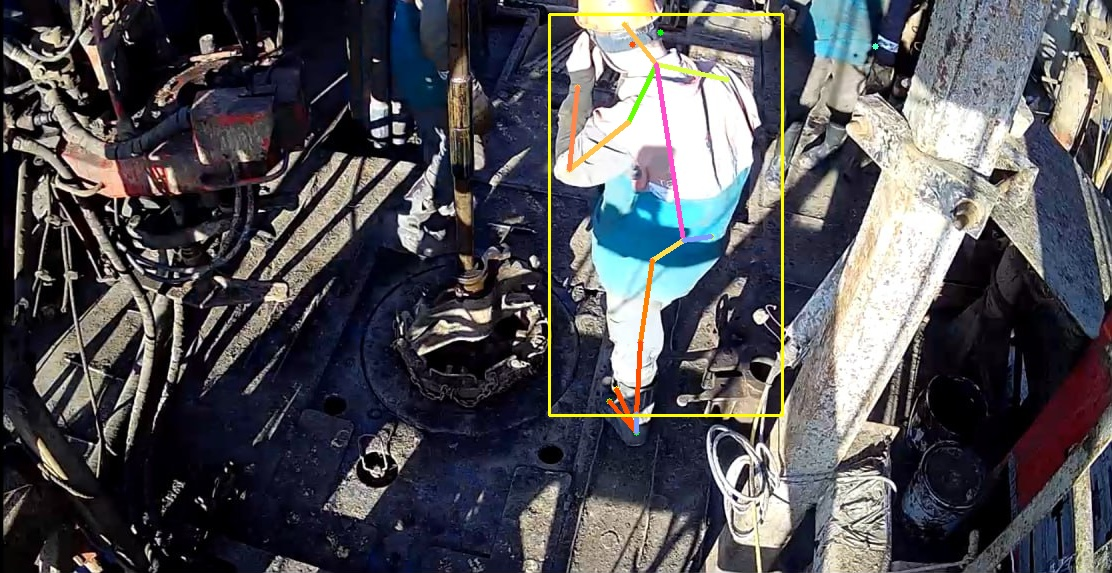
\includegraphics[width=1.0\textwidth,keepaspectratio]{problem_formulation_3}
    \end{figure}
\end{frame}

\begin{frame}
    \frametitle{Постановка задачи}
    Начальные предположения:
    \begin{itemize}
        \item Опасная зона для конкретной камеры задана заранее;
        \item Детектируем только случай нахождения в опасной зоне без СИЗ.
    \end{itemize}

    Список рассматриваемых средств индивидуальной защиты:
    \begin{itemize}
        \item Каска,
        \item Перчатки,
        \item Ботинки.
    \end{itemize}
\end{frame}

\begin{frame}
    \frametitle{Архитектура решения}
    \begin{figure}
        \centering
        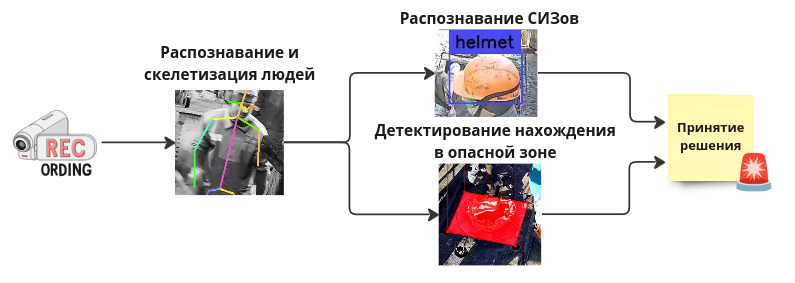
\includegraphics[width=1.1\textwidth,keepaspectratio]{general_architecture}
    \end{figure}
\end{frame}

\begin{frame}
    \frametitle{Цели и задачи}
    Цель работы -- проектирование системы компьютерного зрения для детектирования опасных ситуаций на производстве.

    Задачи работы:
    \begin{enumerate}
        \item Проектирование архитектуры системы компьютерного зрения,
        \item Разработка метода распознавания и скелетизации,
        \item Реализация алгоритма детектирования нахождения в опасной зоне,
        \item Описание принципа принятия решений по заданному кадру.
    \end{enumerate}
\end{frame}
